\documentclass[12pt,letterpaper]{article}
\usepackage{graphicx,textcomp}
\usepackage{natbib}
\usepackage{setspace}
\usepackage{fullpage}
\usepackage{color}
\usepackage[reqno]{amsmath}
\usepackage{amsthm}
\usepackage{fancyvrb}
\usepackage{amssymb,enumerate}
\usepackage[all]{xy}
\usepackage{endnotes}
\usepackage{lscape}
\newtheorem{com}{Comment}
\usepackage{float}
\usepackage{hyperref}
\newtheorem{lem} {Lemma}
\newtheorem{prop}{Proposition}
\newtheorem{thm}{Theorem}
\newtheorem{defn}{Definition}
\newtheorem{cor}{Corollary}
\newtheorem{obs}{Observation}
\usepackage[compact]{titlesec}
\usepackage{dcolumn}
\usepackage{tikz}
\usetikzlibrary{arrows}
\usepackage{multirow}
\usepackage{xcolor}
\newcolumntype{.}{D{.}{.}{-1}}
\newcolumntype{d}[1]{D{.}{.}{#1}}
\definecolor{light-gray}{gray}{0.65}
\usepackage{url}
\usepackage{listings}
\usepackage{color}

\definecolor{codegreen}{rgb}{0,0.6,0}
\definecolor{codegray}{rgb}{0.5,0.5,0.5}
\definecolor{codepurple}{rgb}{0.58,0,0.82}
\definecolor{backcolour}{rgb}{0.95,0.95,0.92}

\lstdefinestyle{mystyle}{
	backgroundcolor=\color{backcolour},   
	commentstyle=\color{codegreen},
	keywordstyle=\color{magenta},
	numberstyle=\tiny\color{codegray},
	stringstyle=\color{codepurple},
	basicstyle=\footnotesize,
	breakatwhitespace=false,         
	breaklines=true,                 
	captionpos=b,                    
	keepspaces=true,                 
	numbers=left,                    
	numbersep=5pt,                  
	showspaces=false,                
	showstringspaces=false,
	showtabs=false,                  
	tabsize=2
}
\lstset{style=mystyle}
\newcommand{\Sref}[1]{Section~\ref{#1}}
\newtheorem{hyp}{Hypothesis}

\title{Problem Set 3}
\date{Yu Fan}
\author{Applied Stats/Quant Methods 1}

\begin{document}
	\maketitle
	\section*{Instructions}
	\begin{itemize}
		\item Please show your work! You may lose points by simply writing in the answer. If the problem requires you to execute commands in \texttt{R}, please include the code you used to get your answers. Please also include the \texttt{.R} file that contains your code. If you are not sure if work needs to be shown for a particular problem, please ask.
	\item Your homework should be submitted electronically on GitHub.
	\item This problem set is due before 23:59 on Sunday November 11, 2024. No late assignments will be accepted.

	\end{itemize}

		\vspace{.25cm}
	
\noindent In this problem set, you will run several regressions and create an add variable plot (see the lecture slides) in \texttt{R} using the \texttt{incumbents\_subset.csv} dataset. Include all of your code.

	\vspace{.5cm}
\section*{Question 1}
\vspace{.25cm}
\noindent We are interested in knowing how the difference in campaign spending between incumbent and challenger affects the incumbent's vote share. 
	\begin{enumerate}
		\item Run a regression where the outcome variable is \texttt{voteshare} and the explanatory variable is \texttt{difflog}.	
			\lstinputlisting[language=R, firstline=38, lastline=40]{my_answer_YuFan.R} 
				\begin{verbatim}
			Call:
			lm(formula = voteshare ~ difflog, data = inc.sub)
			
			Residuals:
			Min       1Q   Median       3Q      Max 
			-0.26832 -0.05345 -0.00377  0.04780  0.32749 
			
			Coefficients:
			Estimate Std. Error t value Pr(>|t|)    
			(Intercept) 0.579031   0.002251  257.19   <2e-16 ***
			difflog     0.041666   0.000968   43.04   <2e-16 ***
			---
			Signif. codes:  0 ‘***’ 0.001 ‘**’ 0.01 ‘*’ 0.05 ‘.’ 0.1 ‘ ’ 1
			
			Residual standard error: 0.07867 on 3191 degrees of freedom
			Multiple R-squared:  0.3673,	Adjusted R-squared:  0.3671 
			F-statistic:  1853 on 1 and 3191 DF,  p-value: < 2.2e-16
			\end{verbatim}  
		\lstinputlisting[language=R, firstline=40, lastline=41]{my_answer_YuFan.R} 
		
		
		The model equation is \( \text{voteshare} = 0.579 + 0.0417 \times \text{difflog} \). The intercept is 0.579, indicating that when difflog is 0, the predicted voteshare is 0.579. The coefficient for difflog is 0.0417, meaning that for every 1-unit increase in difflog, voteshare increases by 0.0417 on average, and this effect is highly significant (p-value < 0.001).\\
		
		The t-value for difflog is 43.04, and the p-value is much smaller than 0.001, indicating a significant positive impact of difflog on voteshare. The F-statistic is 1853, showing the overall significance of the model.\\
		
		The model’s goodness of fit, represented by the R-squared \( R^2 \), is 0.3673, suggesting that difflog explains about 36.73% of the variation in `voteshare`.\\
		
		In conclusion, the difference in logs (difflog) has a significant positive effect on the incumbent's vote share (voteshare). Each unit increase in difflog results in a 0.0417-unit increase in voteshare, with this result being statistically highly significant.\\
		
			\vspace{1cm}
		
		\item Make a scatterplot of the two variables and add the regression line. 
			\lstinputlisting[language=R, firstline=44, lastline=54]{my_answer_YuFan.R}  
				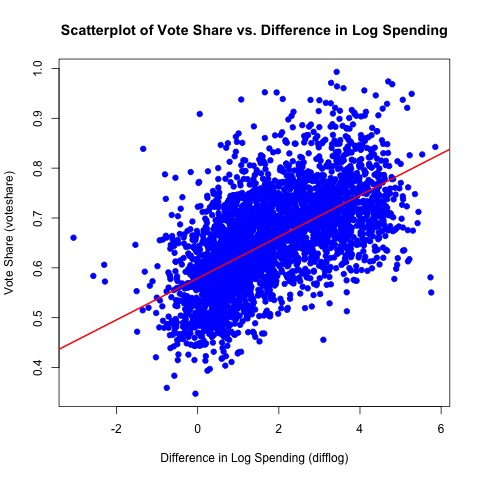
\includegraphics[width=.85\textwidth]{scatterplot_voteshare_difflog.jpg}
			\vspace{7cm}
			
		\item Save the residuals of the model in a separate object.	
			\lstinputlisting[language=R, firstline=57, lastline=64]{my_answer_YuFan.R}  
		\begin{verbatim}
		    1             2             3             4             5             6 
		-0.0004227622 -0.0316840149 -0.0045514943  0.0386688767  0.0355287965  0.0322832521 
		\end{verbatim}  

				
		\item Write the prediction equation.
		
		voteshare=0.579+0.0417×difflog\\
		
		Intercept: 0.579, represents the predicted voteshare when difflog is 0.\\
		difflog coefficient: 0.0417, means that for every unit of difflog, voteshare increases by 0.0417 units.\\

	\end{enumerate}
	
\newpage

\section*{Question 2}
\noindent We are interested in knowing how the difference between incumbent and challenger's spending and the vote share of the presidential candidate of the incumbent's party are related.	\vspace{.25cm}
	\begin{enumerate}
		\item Run a regression where the outcome variable is \texttt{presvote} and the explanatory variable is \texttt{difflog}.
			\lstinputlisting[language=R, firstline=71, lastline=73]{my_answer_YuFan.R}  
				\begin{verbatim}
				Call:
				lm(formula = presvote ~ difflog, data = inc.sub)
				
				Residuals:
				Min       1Q   Median       3Q      Max 
				-0.32196 -0.07407 -0.00102  0.07151  0.42743 
				
				Coefficients:
				Estimate Std. Error t value Pr(>|t|)    
				(Intercept) 0.507583   0.003161  160.60   <2e-16 ***
				difflog     0.023837   0.001359   17.54   <2e-16 ***
				---
				Signif. codes:  0 ‘***’ 0.001 ‘**’ 0.01 ‘*’ 0.05 ‘.’ 0.1 ‘ ’ 1
				
				Residual standard error: 0.1104 on 3191 degrees of freedom
				Multiple R-squared:  0.08795,	Adjusted R-squared:  0.08767 
				F-statistic: 307.7 on 1 and 3191 DF,  p-value: < 2.2e-16
			\end{verbatim}  
			\lstinputlisting[language=R, firstline=74, lastline=74]{my_answer_YuFan.R}  
			 The model equation is:
			\[
			\text{presvote} = 0.5076 + 0.0238 \times \text{difflog}
			\]
			The intercept is 0.5076, indicating that when  difflog is 0, the predicted presvote  is 0.5076. The coefficient for difflog is 0.0238, meaning that for every 1-unit increase in difflog, presvote increases by 0.0238 on average, with this result being statistically highly significant (p-value < 0.001).
			
			The t-value for difflog is 17.54, and the p-value is much smaller than 0.001, indicating a significant positive impact of difflog on presvote. However, the model's goodness of fit is relatively low, with an R-squared \( R^2 \) of 0.08795, suggesting that difflog only explains about 8.8% of the variation in `presvote`.
			
			In conclusion, the difference in logs (difflog) has a significant positive effect on the incumbent party’s presidential vote share (presvote). Each unit increase in difflog results in a 0.0238-unit increase in presvote, but the model has limited explanatory power for the variability in presvote.\\
			
			
		\item Make a scatterplot of the two variables and add the regression line. 
			\lstinputlisting[language=R, firstline=77, lastline=89]{my_answer_YuFan.R}  
				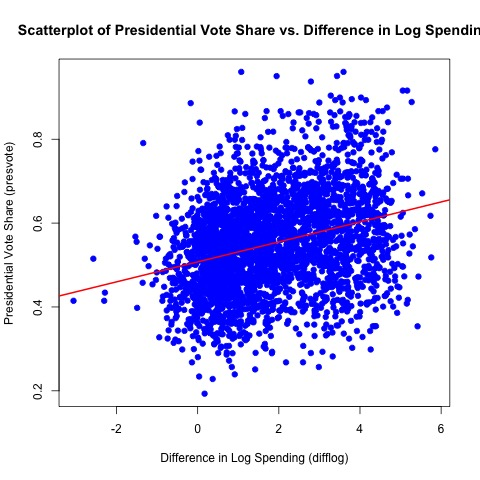
\includegraphics[width=.85\textwidth]{scatterplot_presvote_difflog2.jpg}
			\vspace{5cm}
		
		\item Save the residuals of the model in a separate object.
			\lstinputlisting[language=R, firstline=92, lastline=95]{my_answer_YuFan.R}  
				\begin{verbatim}
			     1            2            3            4            5            6 
			0.005605594  0.037578519 -0.053134788 -0.052993694 -0.045842994  0.074339701 
			\end{verbatim} 
			\vspace{1cm}
			
		\item Write the prediction equation.\\
			presvote=0.5076+0.0238×difflog\\
			
			Intercept: 0.5076, representing the predicted presvote when difflog is 0.\\
			difflog coefficient: 0.0238, indicating that presvote increases by an average of 0.0238 per unit of difflog.\\
	
	\end{enumerate}
	
	\newpage	
\section*{Question 3}

\noindent We are interested in knowing how the vote share of the presidential candidate of the incumbent's party is associated with the incumbent's electoral success.
	\vspace{.25cm}
	\begin{enumerate}
		\item Run a regression where the outcome variable is \texttt{voteshare} and the explanatory variable is \texttt{presvote}.
		\lstinputlisting[language=R, firstline=102, lastline=103]{my_answer_YuFan.R}  
			\begin{verbatim}
			Call:
			lm(formula = voteshare ~ presvote, data = inc.sub)
			
			Residuals:
			Min       1Q   Median       3Q      Max 
			-0.27330 -0.05888  0.00394  0.06148  0.41365 
			
			Coefficients:
			Estimate Std. Error t value Pr(>|t|)    
			(Intercept) 0.441330   0.007599   58.08   <2e-16 ***
			presvote    0.388018   0.013493   28.76   <2e-16 ***
			---
			Signif. codes:  0 ‘***’ 0.001 ‘**’ 0.01 ‘*’ 0.05 ‘.’ 0.1 ‘ ’ 1
			
			Residual standard error: 0.08815 on 3191 degrees of freedom
			Multiple R-squared:  0.2058,	Adjusted R-squared:  0.2056 
			F-statistic:   827 on 1 and 3191 DF,  p-value: < 2.2e-16
		\end{verbatim} 
		\lstinputlisting[language=R, firstline=104, lastline=105]{my_answer_YuFan.R}  
		The model equation is:
		\[
		\text{voteshare} = 0.4413 + 0.3880 \times \text{presvote}
		\]
		The intercept is 0.4413, indicating that when presvote is 0, the predicted voteshare is 0.4413. The coefficient for presvote is 0.3880, meaning that for every 1-unit increase in presvote, voteshare increases by 0.3880 on average, with this result being highly significant (p-value less than 0.001).
		
		The t-value for presvote is 28.76, and the p-value is much smaller than 0.001, showing a significant positive impact of presvote on voteshare. The model’s goodness of fit, represented by the R-squared \( R^2 \), is 0.2058, suggesting that presvote explains about 20.58% of the variation in `voteshare`.
		
		In conclusion, the presidential candidate’s vote share (presvote) has a significant positive effect on the incumbent’s electoral success (voteshare). Each unit increase in presvote results in a 0.3880-unit increase in voteshare. Although the effect is significant, the explanatory power of the variable for the total variation is only 20.58%.
		
			
		\item Make a scatterplot of the two variables and add the regression line. 
		\lstinputlisting[language=R, firstline=108, lastline=120]{my_answer_YuFan.R}  
			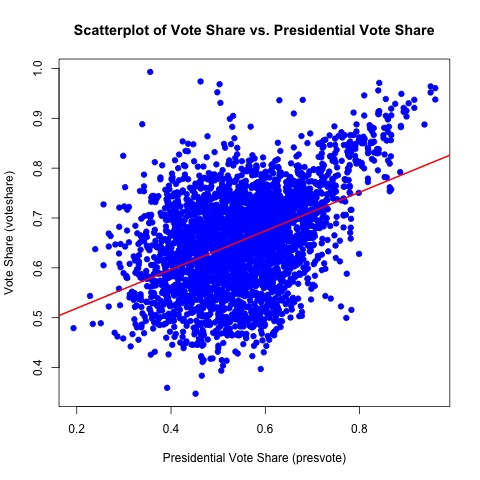
\includegraphics[width=.85\textwidth]{scatterplot_voteshare_presvote3.jpg}
	
			
		\item Write the prediction equation.
	
		Vote Share=0.4413+0.3880×Presvote\\
		
		Intercept: 0.4413, which represents the predicted voteshare when presvote is zero.\\
		presvote coefficient: 0.3880, means that for every unit of presvote, voteshare increases by 0.3880 on average.\\
		
	\end{enumerate}
	

\newpage	
\section*{Question 4}
\noindent The residuals from part (a) tell us how much of the variation in \texttt{voteshare} is $not$ explained by the difference in spending between incumbent and challenger. The residuals in part (b) tell us how much of the variation in \texttt{presvote} is $not$ explained by the difference in spending between incumbent and challenger in the district.
	\begin{enumerate}
		\item Run a regression where the outcome variable is the residuals from Question 1 and the explanatory variable is the residuals from Question 2.
		\lstinputlisting[language=R, firstline=127, lastline=134]{my_answer_YuFan.R}  
		\begin{verbatim}
			Call:
			lm(formula = residuals_question1 ~ residuals_question2)
			
			Residuals:
			Min        1Q    Median        3Q       Max 
			-0.209551 -0.033091  0.001036  0.033227  0.257696 
			
			Coefficients:
			Estimate Std. Error t value Pr(>|t|)    
			(Intercept)         -3.353e-18  9.702e-04    0.00        1    
			residuals_question2  6.401e-01  1.101e-02   58.14   <2e-16 ***
			---
			Signif. codes:  0 ‘***’ 0.001 ‘**’ 0.01 ‘*’ 0.05 ‘.’ 0.1 ‘ ’ 1
			
			Residual standard error: 0.05482 on 3191 degrees of freedom
			Multiple R-squared:  0.5144,	Adjusted R-squared:  0.5142 
			F-statistic:  3380 on 1 and 3191 DF,  p-value: < 2.2e-16
		\end{verbatim} 
		\lstinputlisting[language=R, firstline=135, lastline=135]{my_answer_YuFan.R}  
		The model equation is:
		\[
		\text{residuals\_question1} = -3.353 \times 10^{-18} + 0.6401 \times \text{residuals\_question2}
		\]
		The intercept is -3.353e-18, which is close to 0 and has no statistical significance. The coefficient for esiduals question2 is 0.6401, indicating that for every 1-unit increase in residuals question2, residuals question1 increases by 0.6401 on average, with this result being highly significant (p-value less than 0.001).
		
		The t-value for residuals question2 is 58.14, and the p-value is much smaller than 0.001, showing a significant impact of residuals question2 on residuals question1. The model's goodness of fit, represented by the R-squared \( R^2 \), is 0.5144, suggesting that residuals question2`explains about 51.44% of the variation in `residuals_question1`.
		
		In conclusion, residuals question2 has a significant impact on residuals question1, with the model's explanatory power being 51.44%.
		
		
		\item Make a scatterplot of the two residuals and add the regression line. 	
		\lstinputlisting[language=R, firstline=138, lastline=148]{my_answer_YuFan.R}  
			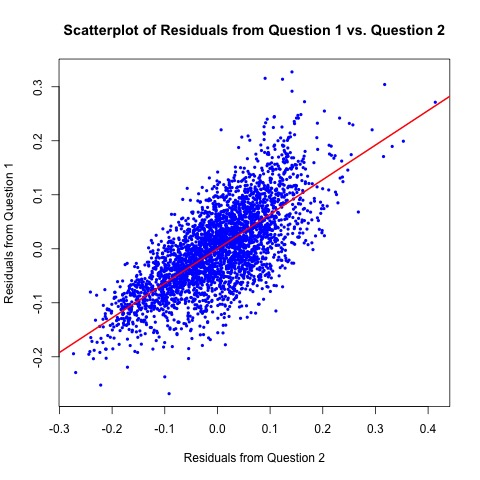
\includegraphics[width=.85\textwidth]{scatterplot_residuals_question1_vs_question2.jpg}
		
		\item Write the prediction equation.

			residuals question1=-3.353e-18+0.6401×residuals question2\\
			
			Intercept: -3.353e-18, close to 0 and therefore negligible.\\
			Coefficient of residuals question2: 0.6401, indicating that residuals question1\\ increases by 0.6401 for every 1 unit increase in residuals question2.\\
	
		
	\end{enumerate}
	\newpage

\section*{Question 5}
\noindent What if the incumbent's vote share is affected by both the president's popularity and the difference in spending between incumbent and challenger? 
	\begin{enumerate}
		\item Run a regression where the outcome variable is the incumbent's \texttt{voteshare} and the explanatory variables are \texttt{difflog} and \texttt{presvote}.	
		\lstinputlisting[language=R, firstline=155, lastline=159]{my_answer_YuFan.R}  
		\begin{verbatim}
			Call:
			lm(formula = voteshare ~ difflog + presvote, data = inc.sub)
			
			Residuals:
			Min       1Q   Median       3Q      Max 
			-0.25928 -0.04737 -0.00121  0.04618  0.33126 
			
			Coefficients:
			Estimate Std. Error t value Pr(>|t|)    
			(Intercept) 0.4486442  0.0063297   70.88   <2e-16 ***
			difflog     0.0355431  0.0009455   37.59   <2e-16 ***
			presvote    0.2568770  0.0117637   21.84   <2e-16 ***
			---
			Signif. codes:  0 ‘***’ 0.001 ‘**’ 0.01 ‘*’ 0.05 ‘.’ 0.1 ‘ ’ 1
			
			Residual standard error: 0.07339 on 3190 degrees of freedom
			Multiple R-squared:  0.4496,	Adjusted R-squared:  0.4493 
			F-statistic:  1303 on 2 and 3190 DF,  p-value: < 2.2e-16
		\end{verbatim} 
		\lstinputlisting[language=R, firstline=160, lastline=160]{my_answer_YuFan.R}  
		The model equation is:
		\[
		\text{voteshare} = 0.4486 + 0.0355 \times \text{difflog} + 0.2569 \times \text{presvote}
		\]
		The intercept is 0.4486, indicating that when both difflog and presvote are 0, the predicted voteshare is 0.4486. The coefficient for difflog is 0.0355, meaning that for every 1-unit increase in difflog, voteshare increases by 0.0355 on average, with this result being highly significant (p-value less than 0.001). The coefficient for presvote is 0.2569, suggesting that voteshare increases by 0.2569 for every 1-unit increase in presvote, also highly significant (p-value less than 0.001).
		
		The p-values for all variables (difflog and presvote) are much smaller than 0.001, indicating significant effects on voteshare. The model's goodness of fit, represented by the R-squared \( R^2 \), is 0.4496, suggesting that difflog and presvote together explain about 44.96% of the variation in `voteshare`.
		
		In conclusion, the incumbent’s vote share (voteshare) is significantly influenced by presidential popularity (presvote) and the spending difference compared to the challenger (difflog). The model indicates that these two factors explain 44.96% of the variation in the incumbent's vote share, with both effects being statistically highly significant.
		
		
		\item Write the prediction equation.	
	
			voteshare=0.4486+0.0355×difflog+0.2569×presvote\\
			
			Intercept: 0.4486, representing the predicted voteshare when both difflog and presvote are 0.\\
			difflog coefficient: 0.0355, indicating that for every unit of difflog, voteshare increases by 0.0355 on average.\\
			presvote coefficient: 0.2569, means that for every unit of presvote, voteshare increases by 0.2569.\\

		
		\item What is it in this output that is identical to the output in Question 4? Why do you think this is the case?
		
			I noticed that some parts were actually pretty similar to what I saw in Question 4. Specifically, the relationship between difflog and voteshare stayed significant, just like before. Also, the p-values for the variables are still showing high significance.\\
			
			So, why is this happening? Well, I think it’s because Question 5’s regression model uses both difflog and presvote together, which gives a more complete explanation of the variation in voteshare. In Question 4, I was looking at how the residuals from voteshare and presvote were related, and here in Question 5, I’m seeing a similar trend. It seems like both factors (difflog and presvote) are strongly connected and influence the incumbent’s vote share together.\\
	
		
	\end{enumerate}




\end{document}
